\documentclass[tikz,border=10pt]{standalone}
\usepackage{tikz}
\usepackage{bm}
\usetikzlibrary{positioning}

\begin{document}
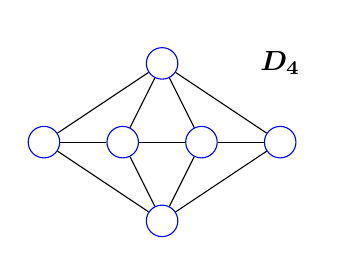
\begin{tikzpicture}[every node/.style={circle, draw, minimum size=4mm, color=blue}]

% A replication of the graph provided in question 5a.

\node (a) at (0,0) {};
\node (b) at (1,0) {};
\node (c) at (2,0) {};
\node (d) at (3,0) {};

\node (e) at (1.5,1) {};
\node (f) at (1.5,-1) {};

\draw (a) -- (b) -- (c) -- (d);

\draw (e) -- (a);
\draw (e) -- (b);
\draw (e) -- (c);
\draw (e) -- (d);

\draw (f) -- (a);
\draw (f) -- (b);
\draw (f) -- (c);
\draw (f) -- (d);

\node[draw=none,text=black] at (3,1) {$\bm{D_4}$};

\end{tikzpicture}
\end{document}